\section{Introduction}

\begin{frame}
  What do researchers do?
\end{frame}

\begin{frame}
  \frametitle{Use, make, and share open results}
  \begin{figure}
    \centering
    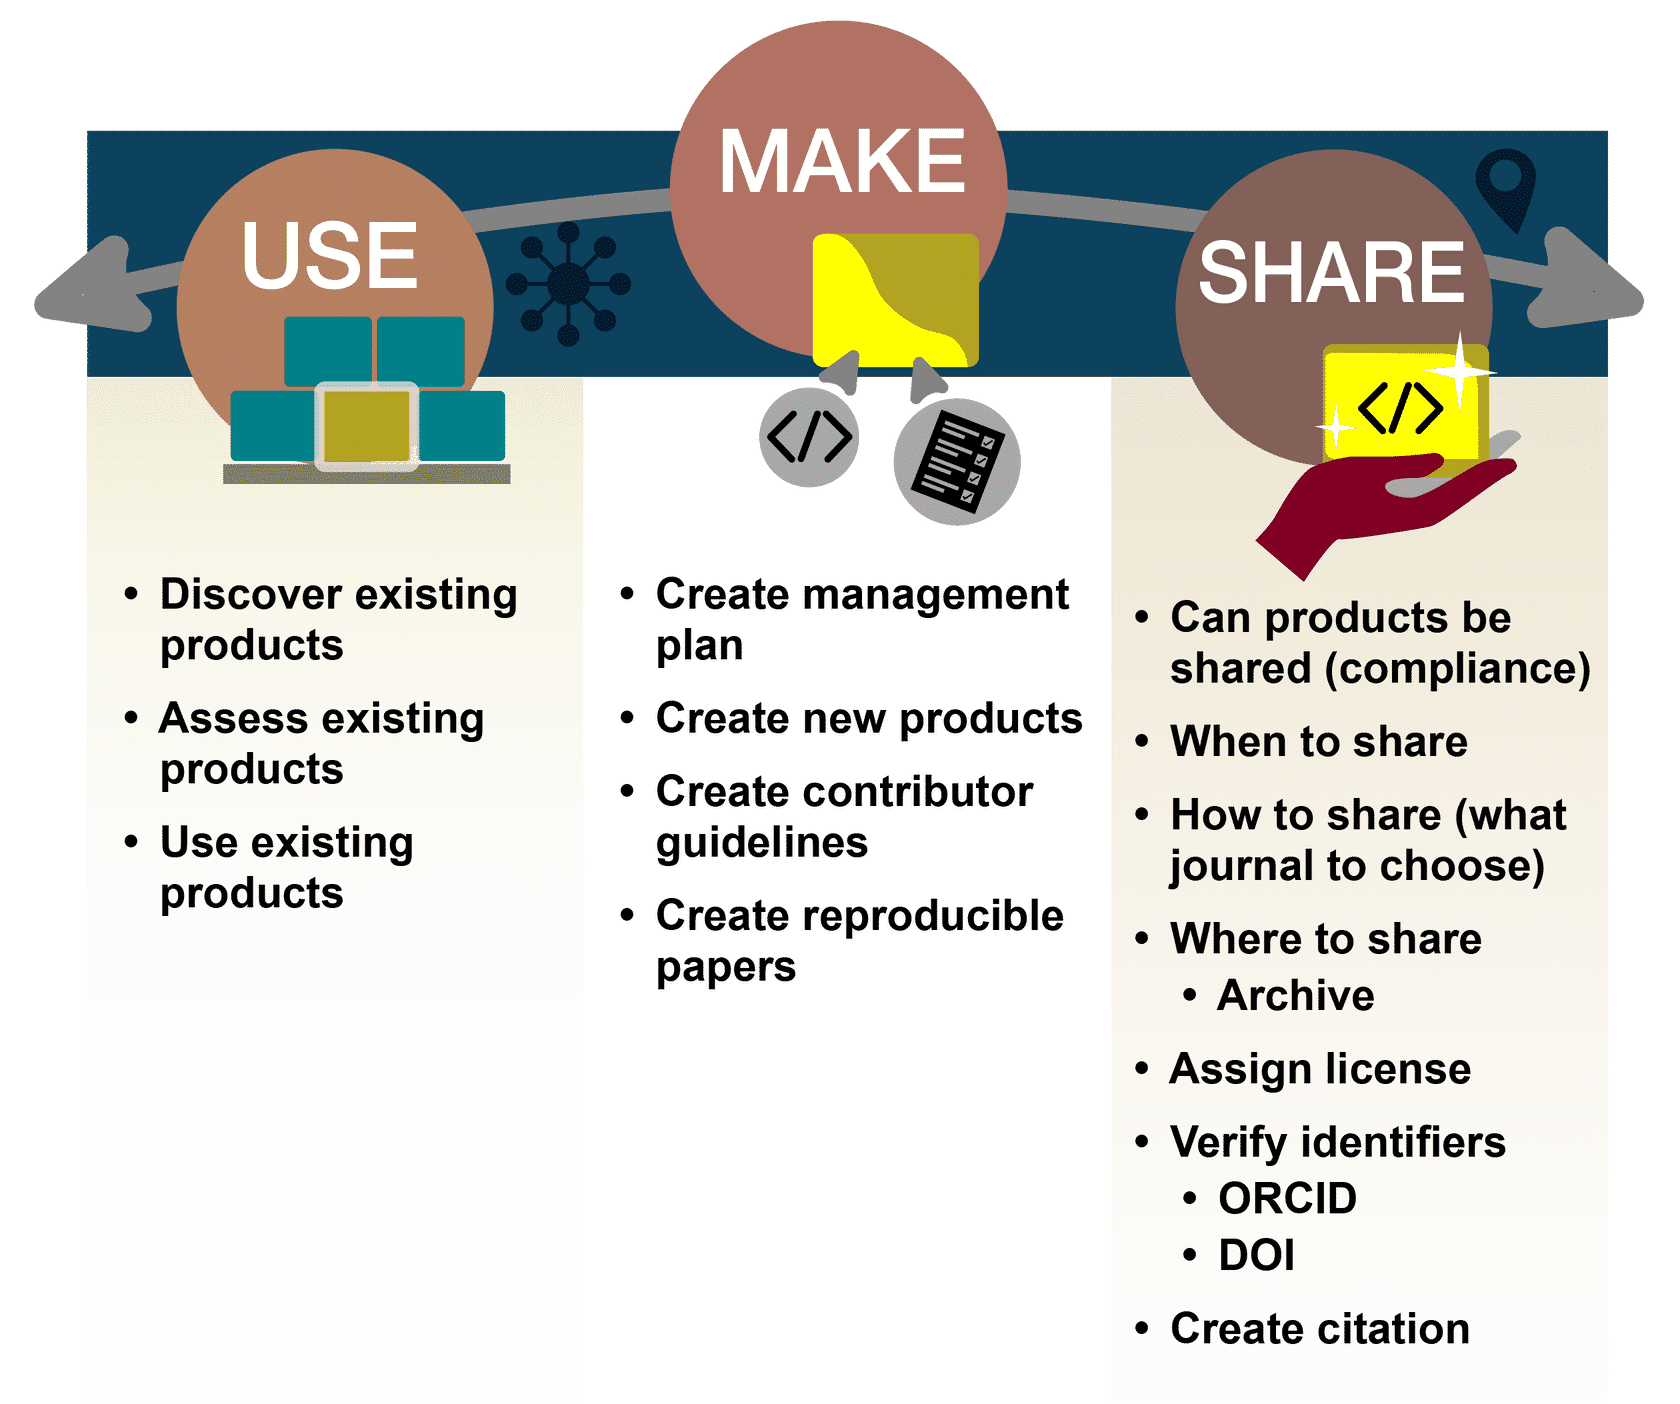
\includegraphics[width=0.5\textwidth]{images/use_make_share.png}
    \label{fig:use_make_share}
    \caption{
Source: \href{https://stemgateway.nasa.gov/s/course-offering/a0BSJ0000049ih3/open-science-101
    }
    {OpenScience101.org}}
  \end{figure}
\end{frame}

\begin{frame}
  \frametitle{The research cycle}
  \begin{figure}
    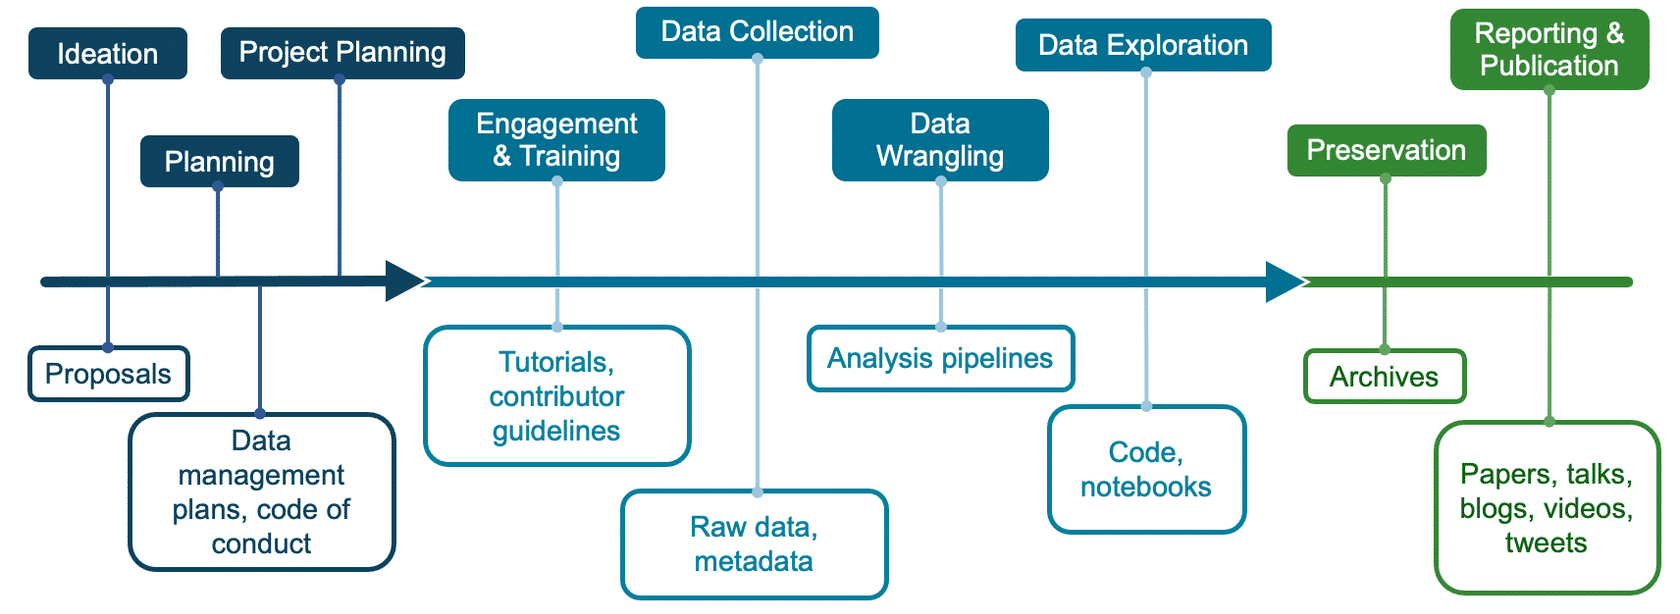
\includegraphics[width=0.9\textwidth]{images/research_cycle.png}
    \label{fig:research_cycle}
    \caption{
Source: \href{https://stemgateway.nasa.gov/s/course-offering/a0BSJ0000049ih3/open-science-101
    }
    {OpenScience101.org}}
  \end{figure}
\end{frame}

\begin{frame}
  \frametitle{Introduction}
  \begin{itemize}
    \item The scientific endeavour is time-consuming.
    \item Scientific research includes, among other tasks, keep track of the
    current scientific literature and use to foster new discoveries.
    \item But also, ensuring the scientific reproducibility of their
    experiments.
    \item Some work related to these task could done using specialized
    software and tools.
  \end{itemize}
\end{frame}

\begin{frame}
  \frametitle{Digital Object Identifier DOI}
  \begin{columns}
    \begin{column}{0.5\textwidth}
      \begin{itemize}
        \item Unique.
        \item Identifier.
        \item Persistent.
        \item Resolvable.
        \item Metadata.
        \item FAIR:
          \begin{itemize}
            \item Findable.
            \item Accessible.
            \item Interoperable.
            \item Reusable.
          \end{itemize}
      \end{itemize}
    \end{column}
    \begin{column}{0.5\textwidth}
      \begin{figure}
        \centering
        
\includegraphics[scale=0.7]{logos/doi_logo.png}
      \end{figure}
    \end{column}
  \end{columns}
\end{frame}
